\documentclass[10pt,xcolor={dvipsnames}]{beamer}
\usepackage[utf8]{inputenc}
\usepackage[czech]{babel}
\usepackage[T1]{fontenc}
\usepackage{amsmath}
\usepackage{amsfonts}
\usepackage{amssymb}
\usepackage{url}
\begin{document}
\title{\textsf{R} - úvod do problematiky}
\author{Lubor Homolka}
\date{\today}
\begin{frame}
\titlepage
\end{frame}

\begin{frame}
\frametitle{Obsah školení}
\begin{large}
Teoretická část:\\
\begin{itemize}
\item[--] Reproducible research \\[0.4cm]
\item[--] R $\sim$ Open-science filosofie \\[0.5cm]
\end{itemize}
Praktická část:\\
\begin{itemize}
\item[--] Literate Coding in R \\[0.4cm]
\item[--] Zdroje a správa dat \\[0.4cm]
\item[--] Vizualizace dat jako příprava pro inferenční statistiku
\end{itemize}
\end{large}
\end{frame}



\begin{frame}[fragile]
\frametitle{Reproducible research}
\begin{Large}
\begin{itemize}
\item[--] \textcolor{WildStrawberry}{RE}\textcolor{NavyBlue}{search}
\item[--] Proč je Reproducible research aktuální téma?
\item[--] váha důkazu $\sim$ p-value?
\end{itemize}
\end{Large}

\end{frame}

\begin{frame}
\frametitle{Literate Coding I}
\Large{Záznam z experimentu}\hrule\bigskip 

Cílem \emph{experimentu} bylo ...\newline
a postupovali jsme následovně:\newline

„Naměřili jsme hodnoty 3,4 a 5 a z nich jsme vypočítali průměr (prostý aritmetický)“ \newline\smallskip

Očekávali jsme, že průměr bude 2, ale nám vyšel 4, což se ale při počtu pozorování dalo očekávat.

\end{frame}

\begin{frame}
\frametitle{Literate Coding II}
\textcolor{NavyBlue}{\Large{Záznam z experimentu}}\hrule\bigskip 

\textcolor{NavyBlue}{Cílem \emph{experimentu} bylo ...\newline
a postupovali jsme následovně:\newline}

\textcolor{WildStrawberry}{„Naměřili jsme hodnoty 3,4 a 5 a z nich jsme vypočítali průměr (prostý aritmetický)“} \newline\smallskip

\textcolor{NavyBlue}{Očekávali jsme, že průměr bude 2, ale nám vyšel} \textcolor{WildStrawberry}{4}, \textcolor{NavyBlue}{což se ale při počtu pozorování dalo očekávat.}\bigskip

\textcolor{NavyBlue}{Běžný text, který je možné psát jazyky: HTML, Markdown nebo \LaTeX.} \newline
\textcolor{WildStrawberry}{„Počítačový jazyk“ - v našem případě R}
\end{frame}

\begin{frame}
\frametitle{Literate Coding III - Knitr}
\begin{figure}
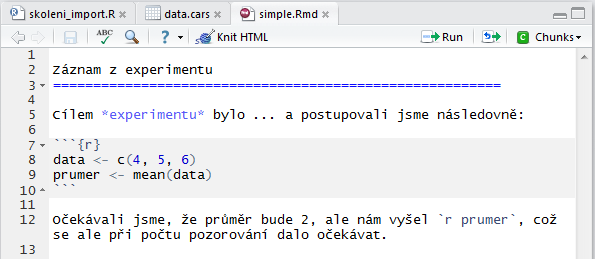
\includegraphics[scale=0.7]{rmarkdown}
\end{figure}
\end{frame}

\begin{frame}
\frametitle{Literate Coding IV - Výsledek}
\begin{figure}
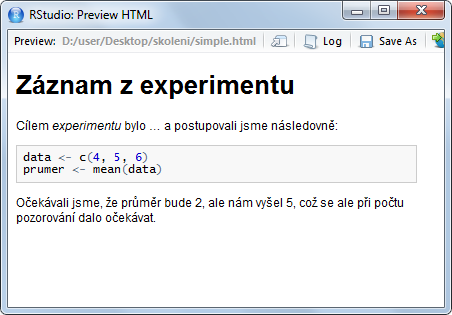
\includegraphics[scale=0.8]{vysledek}
\end{figure}
\end{frame}

\begin{frame}[fragile]
\frametitle{Lokální data I}
\begin{itemize}
\item[--] Ideální zdroj je textový soubor bez \emph{zbytečného} formátování.
\item[--] preferované typy: \texttt{.txt} nebo \texttt{.csv}
\end{itemize}

\textcolor{NavyBlue}{Přihlašte se na \newline
\url{http://www.fame.utb.cz/pokr/}\newline\smallskip
studijni$\_$materialy -> Podniky -> r$\_$skoleni} \newline
a stáhněte si na disk (pracovního adresáře) soubor \texttt{cars.txt}\newline

Načtěte data do R příkazem:
\begin{verbatim}
data.cars <- read.table("cars.txt",sep=" ", header=TRUE)
str(data.cars) #struktura dat
\end{verbatim}
\end{frame}

\begin{frame}[fragile]
\frametitle{Lokální data II}
Další zdroje: \texttt{.xlsx} nebo \texttt{.acddb}
\begin{verbatim}
library(xlsx)
excel.data <- read.xlsx("analyza1.xlsx", sheetIndex=1)
\end{verbatim} 
\end{frame}

\begin{frame}[fragile]
\frametitle{Data z Internetu I}
\texttt{R} umožňuje práci se vzdálenými zdroji, jak „pod heslem“, někdy ale problematické http\textcolor{WildStrawberry}{s}.

\begin{verbatim}
url.cars<-"http://www.stat.ucla.edu/~jeroen/ggplot2/mtcars.txt"
data.cars <- read.table(url.cars,sep=" ", header=TRUE)
write.table(x=data.cars, file="auta.txt", row.names=FALSE)
\end{verbatim} 
\end{frame}

\begin{frame}[fragile]
\frametitle{Data z Internetu II -- \texttt{quantmod}}
\begin{verbatim}
casove.rady <- new.env()
start.date = as.Date("2010-01-11") 
end.date = as.Date("2014-05-04")
akcie <- c("GOOG","UKX")

getSymbols(akcie, env = casove.rady,
	 src = "yahoo",
	 from = startDate,
	 to = endDate)

head(casove.rady$GOOG)
tail(casove.rady$UKX)
plot(casove.rady$UKX)
barChart(casove.rady$UKX)
\end{verbatim} 
\end{frame}

\begin{frame}
\frametitle{Manipulace s daty}
\begin{large}
S daty je možné dělat snad úplně vše i v \texttt{base} knihovně. Práce ale není ani příliš rychlá, ani „elegantní“. \newline\smallskip

Základní funkce:\smallskip
\begin{itemize}
\item[--] \texttt{*apply} a \texttt{order}
\item[--] \texttt{d*ply}, zejména ddply
\end{itemize}
\end{large}
\end{frame}

\begin{frame}
\frametitle{Vizualizace dat}
\begin{large}
\texttt{R} využívá několik knihoven k práci s grafikou. Představíme si základní (base) a dvě rozšíření:
\begin{itemize}
\item[--] \texttt{lattice}
\item[--] \texttt{ggplot2}
\end{itemize}
\end{large}
\end{frame}


\begin{frame}
Prezentace a její obsah je samozřejmě reproducible!
\begin{figure}
\centering

\includegraphics[scale=0.7]{github_logo}
\end{figure}
\url{https://github.com/luboRprojects}
\end{frame}



\end{document}